\section{Recovery Uncertainty, Switch Timing and Alarm Control}
\label{app:recovery-uncertainty-checks}
\newcommand{\NuisanceContrasts}{1\,296}
\newcommand{\NuisanceWorstLoss}{8.4}
\newcommand{\NuisanceRivalChanges}{0}
\newcommand{\SwitchDerivativeError}{1.11\times10^{-7}}
\newcommand{\SwitchMidpointError}{11.67}
\newcommand{\NullMatchedCrossing}{3.57}
\newcommand{\NullShiftedCrossing}{85.66}


\subsection{Uncertainty in the Preceding Load}
After subtracting the mean recovery trajectory, consider a stacked
report vector $r=s_c a+u z+\varepsilon$. Here $s_c$ is the new load
signature, $u$ is the residual trajectory per unit amplitude of a preceding
load, $z\sim\mathcal N(0,\sigma_z^2)$, and
$\varepsilon\sim\mathcal N(0,R)$ is independent of $z$. Let
$W R W^\top=I$ and $v=\sigma_z W u$. For any difference $d$ between
candidate means, the squared distance under the common marginalized
covariance follows from the rank-one inverse identity:
\begin{equation}
 \|d\|^2_{(R+\sigma_z^2uu^\top)^{-1}}
 =\|Wd\|^2-\frac{(v^\top Wd)^2}{1+v^\top v}.
\end{equation}
The loss depends on the alignment with recovery as seen by the PMUs.
With several Gaussian nuisance directions the same construction uses
$R+UKU^\top$. A covariance that varies with the candidate requires the
corresponding quadratic and log-determinant terms for each likelihood.

We used the nominal bank operators, all 47 coordinates, and the common
quiet-null covariance over 30 reports. Each of nine preceding loads
lasts one second and restores using its OFF operator. Each of nine new
loads takes either sign at $0.2\%$ of its setpoint. The four gaps and two
prior scales give \NuisanceContrasts{} deterministic contrasts. Rivals
include all other catalog assets. Load rivals fit their magnitude within
$[-0.2,0.2]$, and line rivals retain fixed signatures. The recovery
direction is shared in each contrast, including against a line rival.
The nearest separation shrinks by at most \NuisanceWorstLoss{}\%;
the nearest rival changes in \NuisanceRivalChanges{} contrasts.
Fig.~\ref{fig:recovery-nuisance} shows the distribution of the losses.
The tested covariance represents one uncertain amplitude, so the result
does not cover uncertainty in the recovery source, timing or plant parameters.

\begin{figure}[t]
\centering
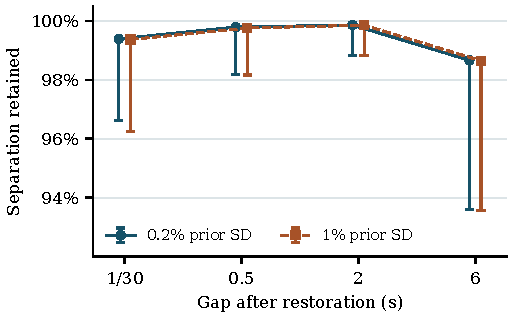
\includegraphics[width=\columnwidth]{figures/generated/recovery_nuisance.pdf}
\caption{Nominal separation retained when the preceding load amplitude is
uncertain. Markers show medians and lower whiskers show tenth percentiles
over 162 deterministic contrasts per gap and prior scale. The horizontal
positions represent four discrete gap settings.}
\label{fig:recovery-nuisance}
\end{figure}

\subsection{Sensitivity Within a Report Interval}
For an affine mode flow with continuous differential state, shifting
a prescribed switch at $\tau$ inserts the sensitivity
$f_-(x_\tau)-f_+(x_\tau)$ at the switch. The subsequent variational
flow propagates that difference \cite{hiskens2000trajectory}. For a
line that opens and recloses, the onset derivative propagates through
both modes. The restoration derivative starts at the second switch.
The algebraic observation map is fixed on each open interval between
reports and changes when a candidate switch crosses a report.

We checked both derivatives on the saved nominal and line 23--24
operators using the eight PMU voltages in rectangular coordinates.
Four noiseless cases generated and fitted with the same model place
both switches off the report grid. Central differences agree with
the derivatives to a maximum relative error of
$\SwitchDerivativeError$. Starting at the interval midpoints gives
errors up to \SwitchMidpointError{}\,ms. Fitting within the supplied
intervals recovers both switch times to within $0.01$\,ms in all four
cases. Timing and asset search, model mismatch, and measurement noise
remain outside this derivative check.

\subsection{Sequential Evidence Under Null Mismatch}
For normalized predictive densities $q_t$ and $p_{0,t}$ selected from
past reports, the product of $q_t(y_t)/p_{0,t}(y_t)$ is a nonnegative
martingale under a correctly specified null with common support.
Ville's inequality bounds the probability of ever crossing $1/\alpha$
by $\alpha$ for one test starting at one \cite{howard2020timeuniform}. This probability refers to
the full test and differs from the published alarm count per hour.

We illustrate the dependence on the null in 20,000 simulated sequences
of 120 independent Gaussian reports. The numerator is
$\mathcal N(0.5,1)$ and the denominator is $\mathcal N(0,1)$.
At $\alpha=0.05$, \NullMatchedCrossing{}\% of matched-null sequences
cross the threshold. With the same noise draws and an unmodeled
$0.35$ shift of the actual null mean, \NullShiftedCrossing{}\% cross.
The shift changes the expected log increment from $-0.125$ to $0.05$.
The example motivates checking the normal predictive law before using
a sequential guarantee for PMU monitoring.\EOD
